% Author: Thomas Klee
% Last revised: 2019-01-15

% typeset with LaTeX only; no need for Bibtex on this file unless references needed

% Preamble
\documentclass{beamer}
\usetheme{Singapore}
%\usetheme{Dresden}
\usefonttheme[onlysmall]{structurebold}
\setbeamerfont{title}{shape=\itshape,family=\rmfamily}
\usepackage{graphicx}
\usepackage[english]{babel}
\usepackage[utf8x]{inputenc}
\usepackage{amsmath}
\usepackage{amsfonts}
\usepackage{amssymb}
\usepackage{xcolor}
\usepackage{booktabs}
\usepackage{ctable} % for command-driven tables

% activate following line for custom appearance
% \usepackage{beamerthemesplit} 

\mode<presentation>

% information for title slide
%\title{\emph{Welcome to \dots}}
\title{Welcome to \dots}
\subtitle{}
\author{Evidence-Based Practice in Speech-Language Therapy \\ (SHSC 2033)}
\institute{Session 1}
\date{Thomas Klee \& Elizabeth Barrett}
\titlegraphic{
\includegraphics[width=6cm]{images/logo_CE_C.jpg}} % HKU logo

\begin{document}

% create title slide with information above
\begin{frame}
	\titlepage
\end{frame}

\section*{Introduction}

% Section break
\begin{frame}
\begin{center}
\Huge{Introduction}
\end{center}
\end{frame}

% 1
\begin{frame}{Should we believe this?}
	\begin{columns}[T]
		\begin{column}{.5\textwidth}
			\begin{block}{CNN website, 12/2016} 
			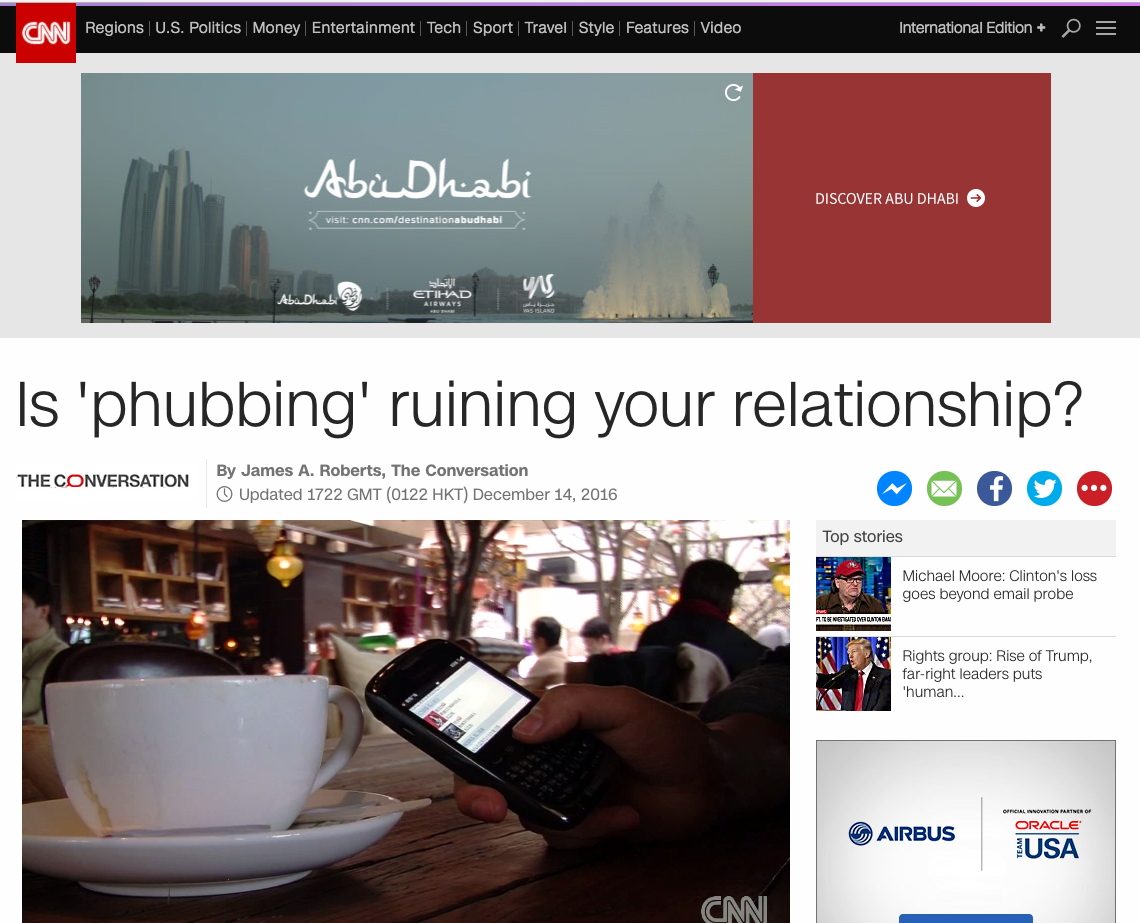
\includegraphics[width=5cm]{images/phubbing_2016.png}
			\end{block}
		\end{column}
		\begin{column}{.5\textwidth}
			\begin{block}{Phubbing (\emph{phone} + \emph{snubbing})} 
			\emph{``How often your romantic partner is distracted by his or her smartphone in your presence"} \\
			\end{block}
 			\begin{block}{Claim:}
			\emph{``70\% of participants said that phubbing hurt their ability to interact with their romantic partners."}
			\end{block}
		\end{column}
	\end{columns}
\end{frame}

% 2
\begin{frame} {What about these?}
	\begin{center}
	\includegraphics[width=.9\textwidth]{images/metro.pdf}
	\end{center}
\end{frame}

% 3
\begin{frame} {How would you respond if your client asked you about the McGuire Programme?}
	\begin{center}
	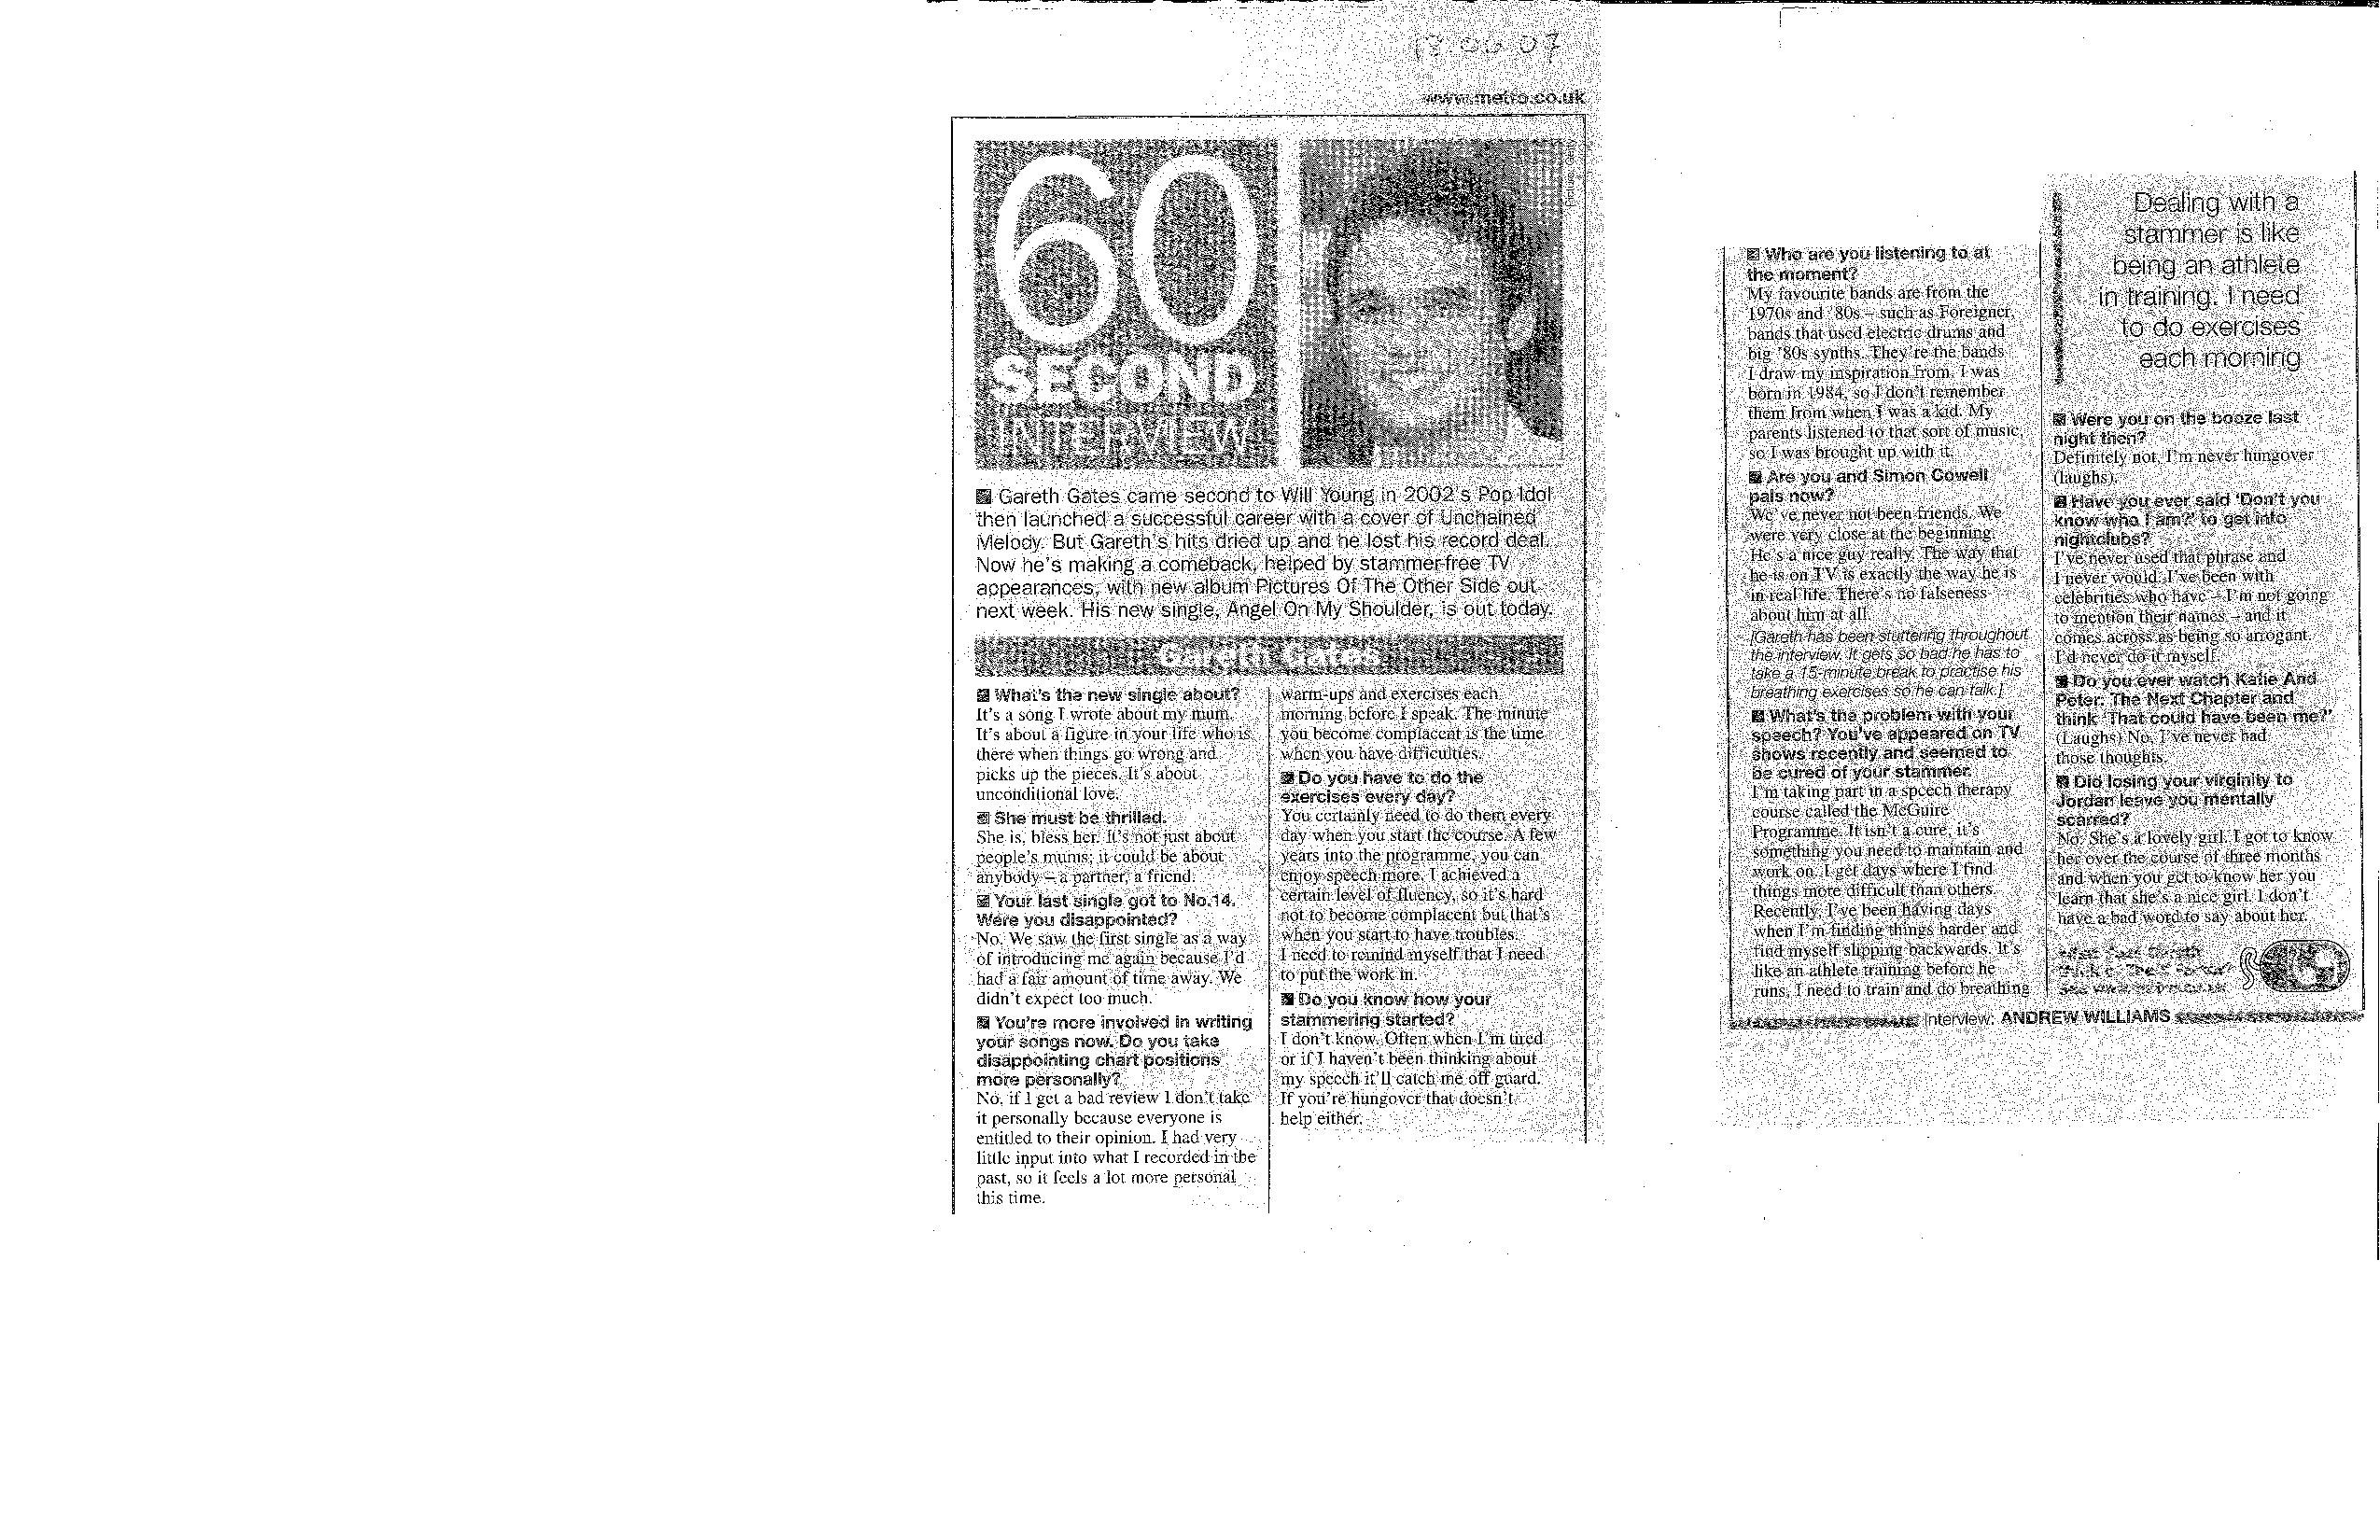
\includegraphics[width=.8\textwidth]{images/gareth_gates.pdf}
	\end{center}
\end{frame}

% 4
\begin{frame} {Would you ask your employer to fund these?}
	\begin{center}
	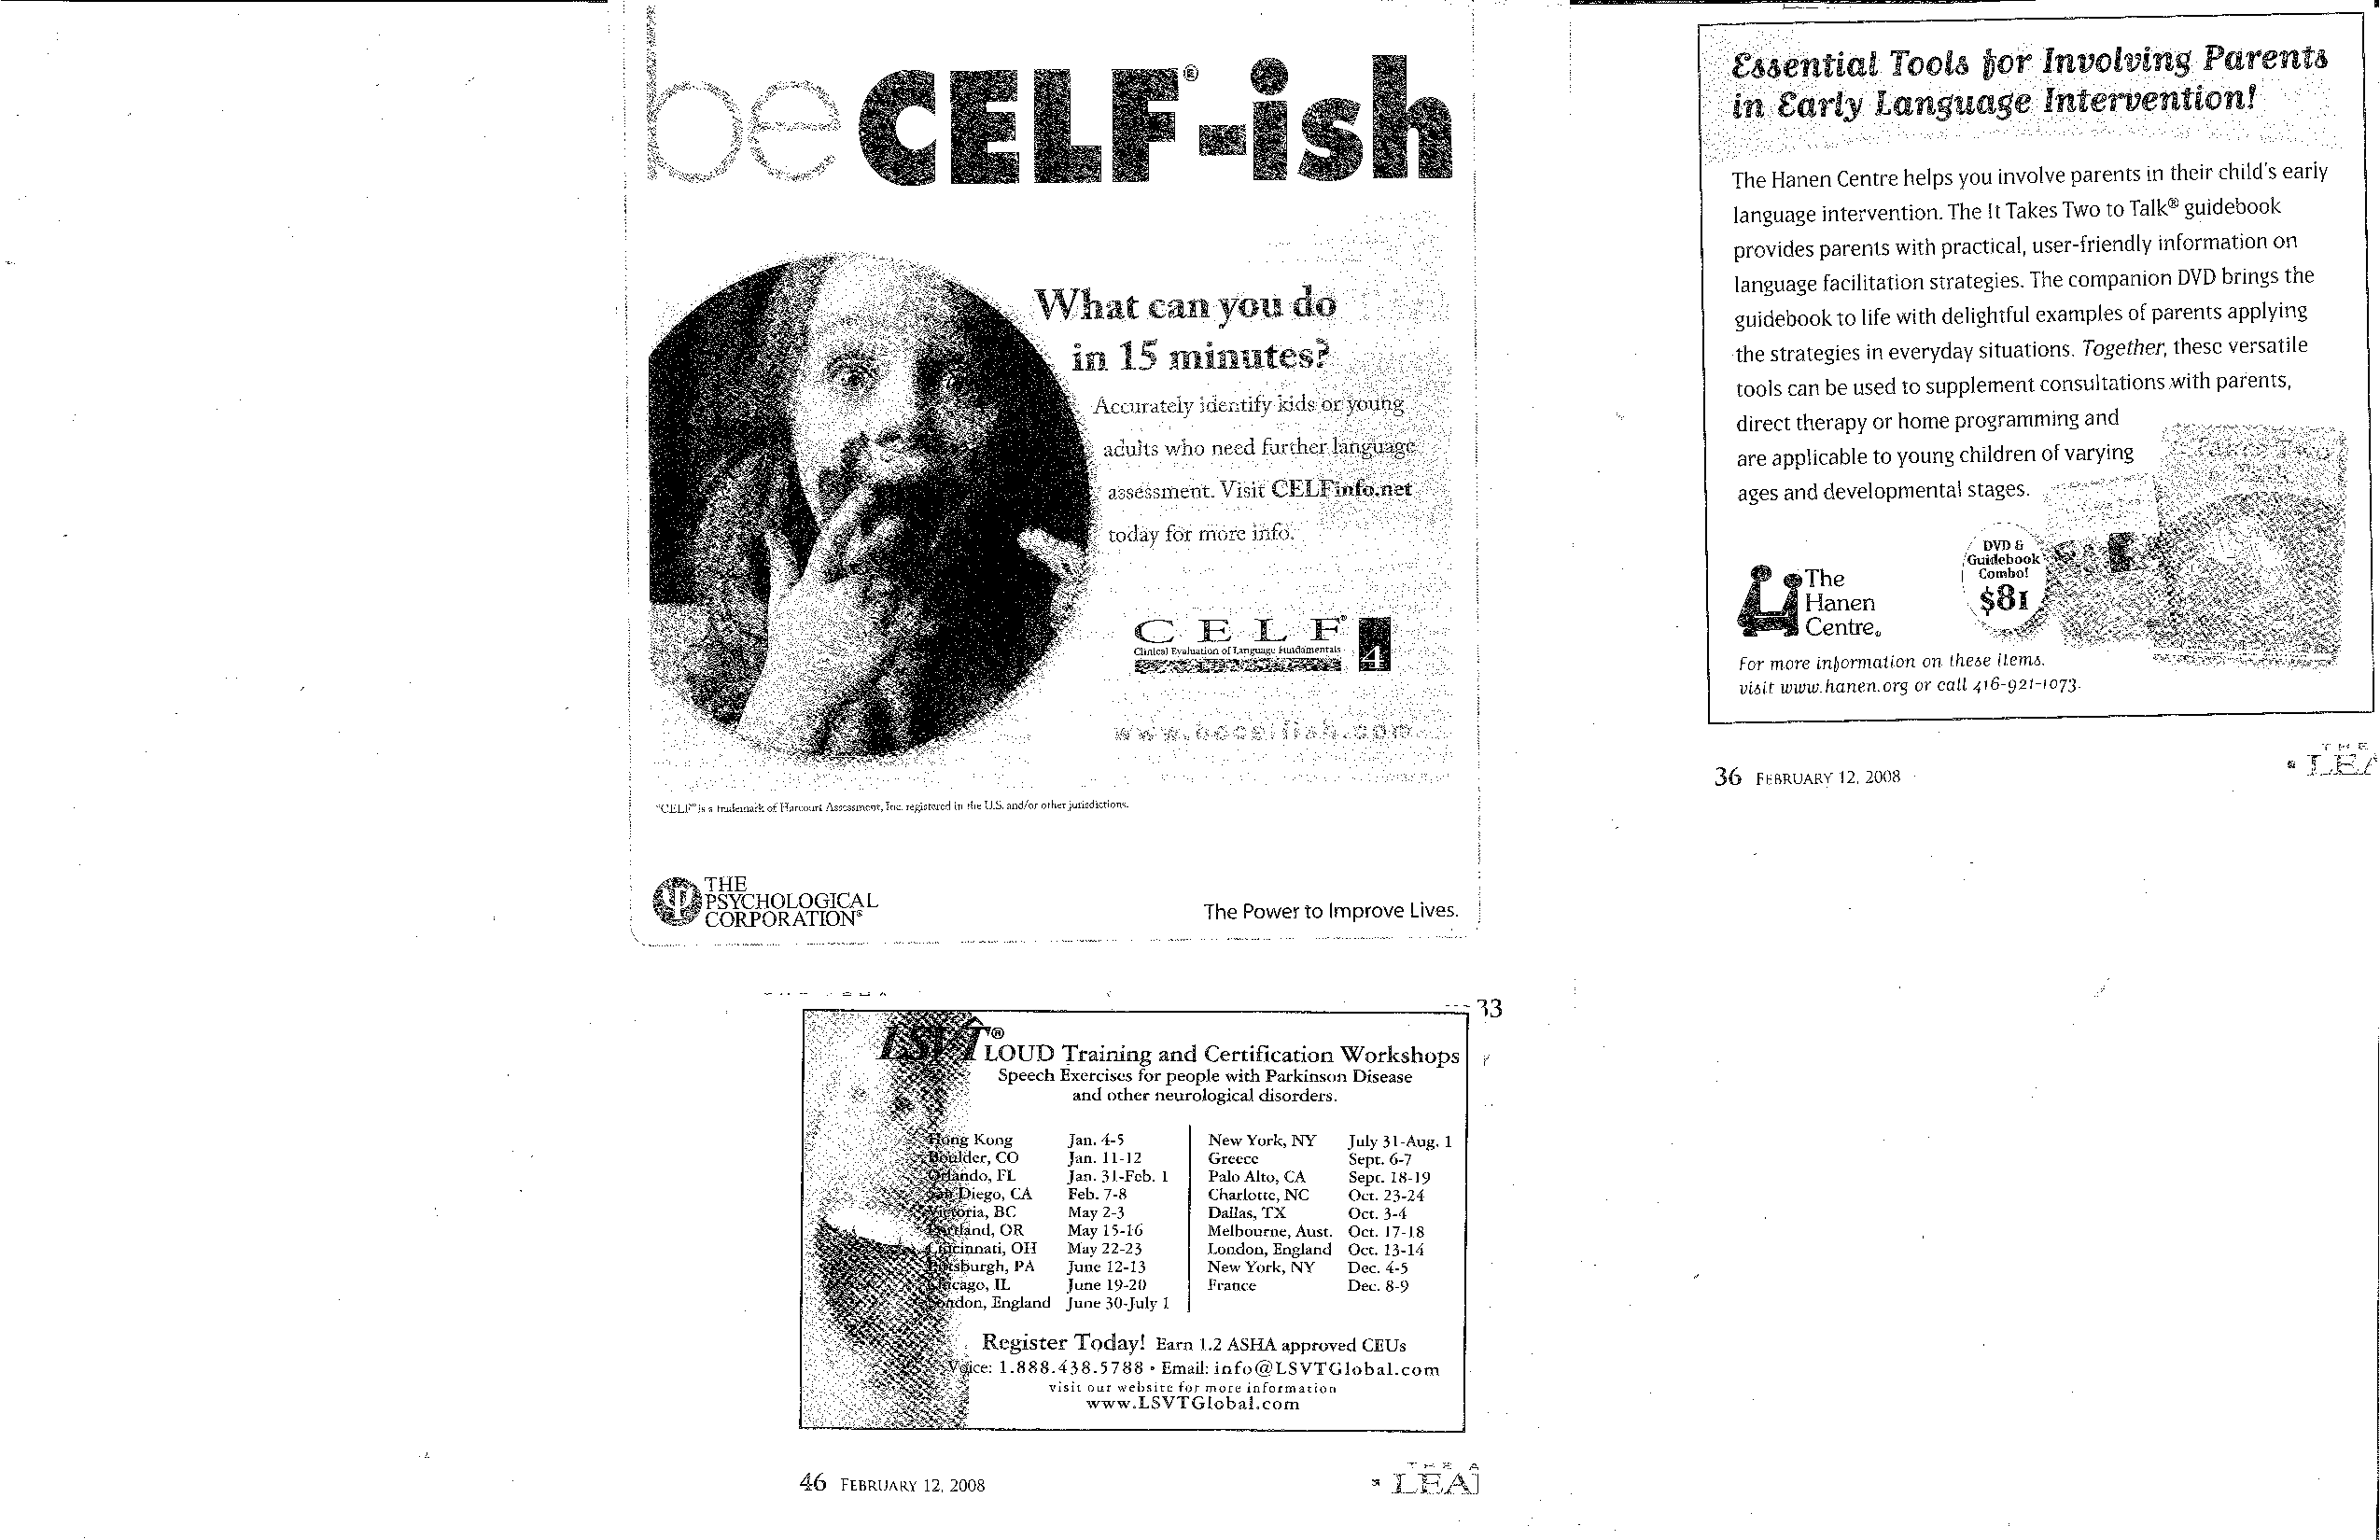
\includegraphics[width=1.0\textwidth]{images/ASHALeader.pdf}
	\end{center}
\end{frame}

\section*{The Course}

% section break
\begin{frame}
\begin{center}
\Huge{The Course}
\end{center}
\end{frame}

% 5
\begin{frame}{Outline}
	\begin{enumerate}
	\item The course: what to expect and what is expected of you
	\item What is evidence-based practice?
	\item Asking clinical questions
	\item Searching for the best evidence
	\item Practical session
		\begin{itemize}
		\item Kendy Lau, Education Librarian
		\item 11am--12.20pm
		\end{itemize}
	\end {enumerate}
\end{frame}

% 6
\begin{frame}{What this course is about}
Provide a framework and tools to help you develop your ability to think critically about clinical intervention and assessment. You will learn to: \\
	\begin{itemize}
	\item Formulate answerable clinical questions
	\item Search the literature for the best evidence available
	\item Critically appraise the research evidence
	\item Synthesise the best evidence to answer the clinical question
	\item Compare the highest-quality evidence to existing clinical practice and decide if a change is necessary
	\item Consider your client's values and preferences in relation to the evidence
	\end{itemize}
\end{frame}

% 7
\begin{frame}{What this course is not about\dots}
	\begin{itemize}
	\item You won't learn what kind of intervention works best for specific types of communication/swallowing disorder.
	\item You won't learn which clinical assessments work best -- and which should be avoided.
	\end{itemize} 
\end{frame}

% 8
\begin{frame}{What is expected of you}
The REALLY BIG CHALLENGES \\
	\begin{itemize}
	\item Recognise that we all are biased in our thinking.
	\item Be open to changing what you think in light of new evidence.
	\end{itemize}
\end{frame}

% 9
\begin{frame}{What is expected of you}
The annoying things
	\begin{itemize}
	\item Attend class; be there on time.
	\item Read what is the required \alert{before} you come to class -- and upload a short summary of the required seminar reading to Moodle \alert{before} the start of each class.
	\item Actively participate in small group discussions.
	\item Complete four quizzes at the beginning of randomly-chosen classes.
	\item Complete two written assignments.
	\end{itemize}
\end{frame}

% 10
\begin{frame}{Course textbook}
	\begin{itemize}
	\item Dollaghan, C.A. (2007). \emph{The handbook for evidence-based practice in communication disorders.} Baltimore, MD: Paul H. Brookes Publishing Co. (main textbook)
	\item Greenhalgh, T. (2010). \emph{How to read a paper: the basics of evidence-based medicine (4th ed.).} Chichester: Wiley-Blackwell BMJ Books. (excellent alternative for further information)
	\end{itemize}
\end{frame}

% 11
\begin{frame}{Class sessions}
	\begin{enumerate}
	\item \textbf{Lecture} based on required readings 
	\item Break
	\item \textbf{Small group, seminar discussion} based on required readings and completion of critical appraisal forms
	\item \textbf{Summing up} at the end
	\end{enumerate}
\end{frame}

\section*{Definitions}

% section break
\begin{frame}
\begin{center}
\Huge{Definitions}
\end{center}
\end{frame}

% 12a
\begin{frame}{What is EBP?}
	\begin{quote}
	``\dots the conscientious, explicit and judicious use of current best evidence in making decisions about the care of individual patients. The practice of evidence based 		medicine means integrating individual clinical expertise with the best available external clinical evidence from systematic research.''  (Sackett et al 1996: 71)
	\end{quote}
\end{frame}

% 12b
\begin{frame}{What is EBP?}
	\begin{quote}
	``\dots the conscientious, explicit and judicious use of current best evidence in making decisions about the care of individual patients. The practice of evidence based 		medicine means \textcolor{blue}{integrating individual clinical expertise} with the \textcolor{red}{best available external clinical evidence from systematic 			research.}" (Sackett et al 1996, p. 71)
	\end{quote}
\end{frame}

% 13
\begin{frame}{Changes to the definition over time}
	\begin{quote}
	``\dots the integration of the best research evidence with clinical expertise and patient values" (Sackett et al 2000, p. 1)
	\end{quote}
	
	\begin{quote}
	``\dots the integration of the best research evidence with our clinical expertise and our patient's unique values and circumstances" (Straus et al 2005, p. 1)
	\end{quote}
\end{frame}

% 14a
\begin{frame}{Evidence-Based Practice ({E$^3$BP})}
	\begin{quote}
	``\dots the conscientious, explicit, and judicious integration of best available\\
		\begin{enumerate}
		\item external evidence from systematic research,
		\item evidence internal to clinical practice, and
		\item evidence concerning the preferences of a fully informed patient." (Dollaghan, 2007, p. 2)
		\end{enumerate}
	\end{quote}
\end{frame}

% 14b
\begin{frame}{\alert{Evidence-}Based Practice ({E$^3$BP})}
	\begin{quote}
	``\dots the conscientious, explicit, and judicious integration of  best available\\
		\begin{enumerate}
		\item external \alert{evidence} from systematic research,
		\item \alert{evidence} internal to clinical practice, and
		\item \alert{evidence} concerning the preferences of a fully informed patient." (Dollaghan, 2007, p. 2)
		\end{enumerate}
	\end{quote}
\end{frame}

% 15
\begin{frame}{And to be honest\dots}
	\begin{quote}
	``\dots the use of mathematical estimates of the risk of benefit and harm, derived from high-quality research on population samples, to inform clinical decision making in the diagnosis, investigation or management of individual patients." (Greenhalgh 2010, p. 1)
	\end{quote}
\end{frame}

\section*{Asking Clinical Questions}

% section break
\begin{frame}
\begin{center}
\Huge{Asking Clinical Questions}
\end{center}
\end{frame}

% 16
\begin{frame}{Asking clinical questions: PICO format}
	\begin{description}
	\item[P] defines the Patient or the Problem
	\item[I] defines the Intervention
	\item[C] describes the Comparison group
	\item[O] describes the clinical Outcome (Haynes et al 2006, p. 11)
	\end{description} 
\end{frame}

% 17
\begin{frame}{PICO question 1}
	\begin{description}
	\item[Patient] For adults who stutter,
	\item[Intervention] does the McGuire Programme
	\item [Outcome] lead to a significant improvement in self-reported stuttering behaviour\footnote{\scriptsize{Outcome measure: OASES self-report questionnaire (Yaruss \& Quesal 2006)}}
	\item[Comparison] compared to no intervention?
	\end{description}
\end{frame}

% 18
\begin{frame}{PICO question 2}
	\begin{description}
	\item[Patient] For children who stutter,
	\item[Intervention] does the Lidcombe Programme
	\item[Outcome] lead to a significant reduction in the proportion of syllables stuttered
	\item[Comparison] compared to other interventions?
	\end{description}
\end{frame}

\section*{Searching for Evidence}

% section break
\begin{frame}
\begin{center}
\Huge{Searching for Evidence}
\end{center}
\end{frame}

% 19
\begin{frame} {Searching for the best evidence}
	\begin{itemize}
	\item Google
	\item Google Scholar: \url{https://scholar.google.com.hk/}
	\item Specialised on-line databases: 
		\begin{itemize}
		\item[-] PubMed \\ \url{https://www.ncbi.nlm.nih.gov/pubmed}
		\item[-] Trip (Turning Research Into Practice) \\ \url{https://www.tripdatabase.com/}
		\item[-] Cochrane Library \\ \url{http://www.cochranelibrary.com/}
		\item[-] PsychINFO \\ \url{http://www.apa.org/pubs/databases/psycinfo/} 
		\item[-] CINAHL \url{https://health.ebsco.com/products/the-cinahl-database}
		\end{itemize}
	\item MeSH terms (PubMed, Medline)
	\end{itemize}
\end{frame}

% 20
%\begin{frame} {Next: a practical session}
%	\begin{itemize}
%	\item Main Library, E-learning Lab, G/F
%	\item 11am--12.20pm
%	\end{itemize}
%\end{frame}

\end{document}